\chapter{A typology of street patterns}
\label{chap:typology}


Street networks of cities can be thought as a simplified schematic view of
cities, which however captures a large part of their structure and organization
\cite{Southworth:2003}.  Despite their apparent diversity, underlying universal
mechanisms are certainly at play in the formation and evolution of street
networks and extracting common patterns between cities is a way towards their
identification. This program is not new \cite{Haggett:1969}, but the
recent dramatic increase  of data availability such as digitized maps,
historical or
contemporary~\cite{Strano:2012,Barthelemy:2013,Porta:2014}\graffito{OpenStreetMap
data are freely available at \url{www.openstreetmap.org}} allows now to test
ideas and models on large scale cross-sectional and historical data.\\

Streets form a network which to a good approximation is planar (where nodes are
intersections and links are segment roads) and which is now fairly well
characterized
\cite{Jiang:2004,Roswall:2005,Porta:2006,Porta:2006b,Lammer:2006,Crucitti:2006,Cardillo:2006,Xie:2007,Jiang:2007,Masucci:2009,Chan:2011,Courtat:2011}.
Due to spatial constraints, the degree distribution is peaked, the clustering
coefficient and assortativity are large, and most of the interesting information
lies in the spatial distribution of betweeenness centrality
\cite{Barthelemy:2011}. It is then tempting to use this information to compare
various cities with each other and to provide a classification. \\

The problem, from a fundamental point of view is however difficult: finding a
typology of street patterns amounts essentially to classify planar graphs, a non
trivial problem. For street networks, this problem has been addressed by the
space syntax community \cite{Hillier,Penn} and a good account can be found in
the book by Marshall~\cite{Marshall:2006}. These works, although based on
empirical observations, contain a large part of subjectivity and our goal is to
eliminate this subjective part to reach a non ambiguous, scientific
classification of these patterns. An interesting direction was provided in the
study of leaves and their classification according to their veination patterns
\cite{Katifori:2012,Weitz:2012}, but with a notable difference which prevents us
from a direct application to streets and which is the existence of a hierarchy
of veins governed by their diameter. From a mathematical point of view there
exists an exact bijection between planar graphs and trees \cite{BDG} which
provides an interesting direction. Using this bijection, classifying planar
graphs would amount to classify trees, which is a simpler problem. However, this
bijection does not take into account the geometrical shape of the planar graph:
indeed two street patterns can have the same topology but cells could be of very
different areas, leading to patterns visually different and to cities of
different structure. It is thus important to take into account not only the
topology of the planar graph --- as described by the adjacency matrix --- but
also the position of the nodes. In order to do that, we propose in this article,
a method to characterize this complex object by extracting the `fingerprint' of
a street pattern. These fingerprints allow us to define a measure of the
distance between two graphs and to construct a classification of cities.


\section{Streets versus blocks}

A major shortcoming of existing classifications  is that they are mostly based
on the street network. This is however problematic, for two different reasons.
First, there is no unambiguous, purely geometrical definition of what a street
is: we could define it as the road segment between two intersections, as an
almost straight line (up to a certain angular tolerance, see \cite{Con}), or we
could also follow the actual street names. There is a certain degree of
arbitrariness in each of these definitions, and it is not clear how robust a
classification based on streets would be. Second, it seems that what is
perceived by the human eye of a city map is not coming from streets but from the
distribution of the shape, area and disposition of blocks (see
Fig.~\ref{fig:example}). 

\begin{figure}
    \centering
    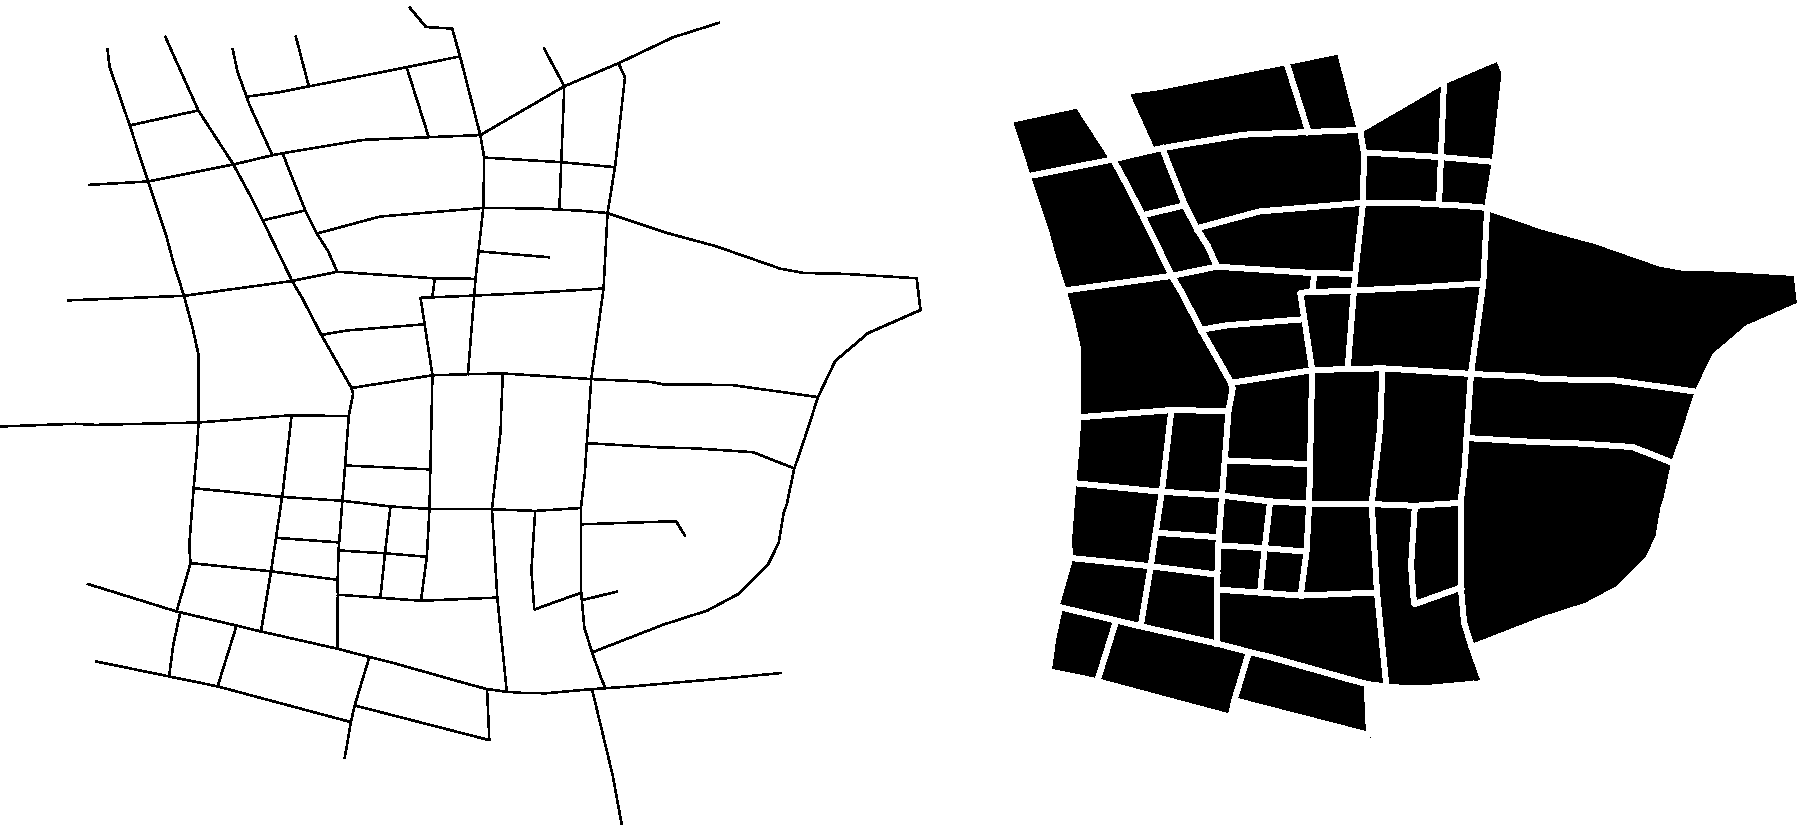
\includegraphics[width=0.7\textwidth]{./gfx/chapter-networks/example.pdf}
    \caption{{\bf From the street network to blocks.} Example of a street pattern
    taken in the neighbourhood of Shibuya in Tokyo (Japan) and the corresponding set
    of blocks. Note that the block representation does not take into account
    dead-ends.  \label{fig:example}} 
\end{figure}

A natural idea when trying to classify cities is thus to focus on blocks (or
cells, or faces) rather than streets. A block can usually be defined without
ambiguity as being the smallest area delimited by roads (it has then to be
distinguished from a parcel which is a tax related definition). While the
information contained in the blocks and the streets are equivalent (up to
dead-ends), the information related to the visual aspect of the street network
seems to be easier to extract from blocks which are simple geometrical objects
--- polygons --- whose properties are easily measured. The block seems then to
be a good candidate for attempting a classification of city patterns. 


\section{Characterizing blocks}

Blocks are defined as the cells of the planar graph formed by streets, and it is
relatively easy to extract them from a map. We have gathered road networks for
$131$ major cities accross the world, spanning all continents (but Antartica),
and their locations are represented on the map Fig.~\ref{fig:world_map}. The
street networks have been obtained from the OpenStreetMap database \cite{OSM},
and restricted to the city center using the Global Administrative Areas database
(or databases provided by the countries administration). We extracted the blocks
from the street network and cleaned undesired features. We end up with a set of
blocks, each with a geographical position corresponding to their centroids. 

\begin{figure}
    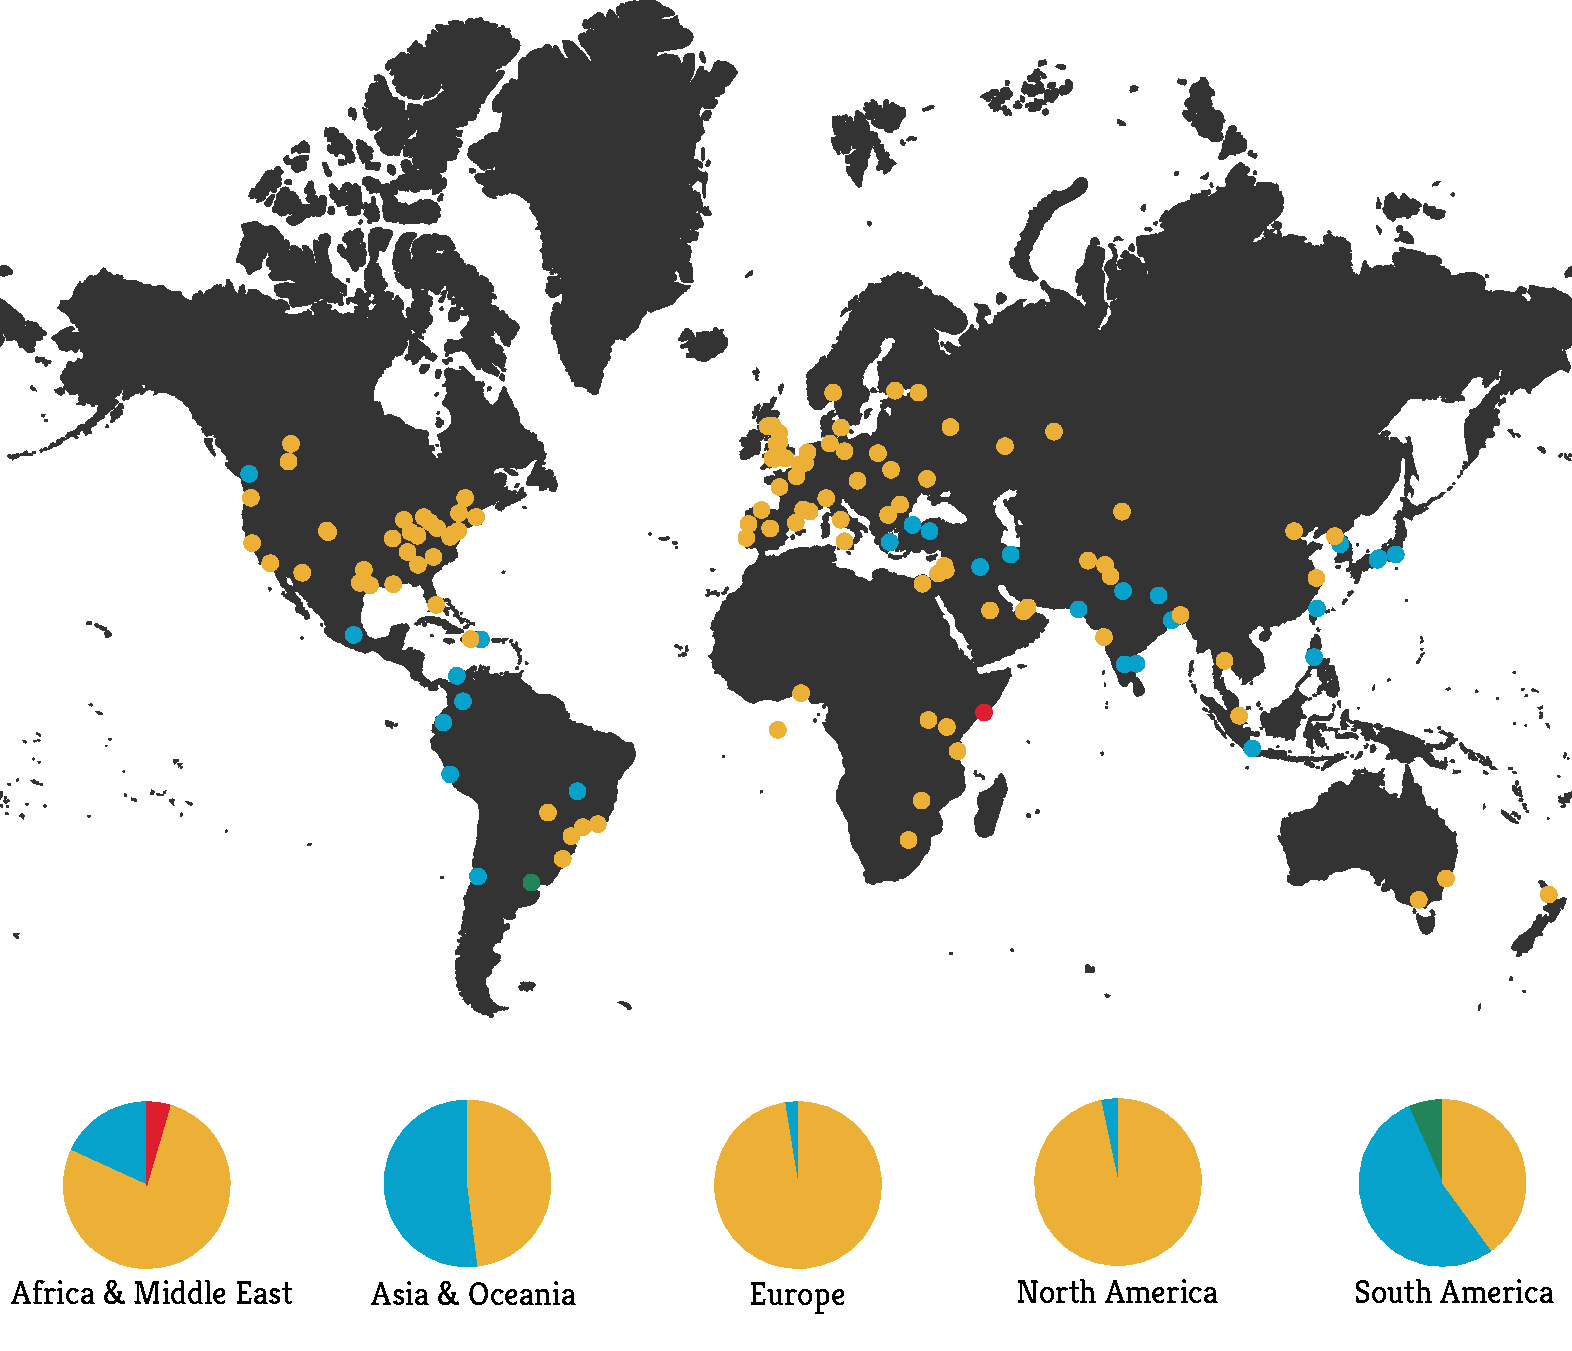
\includegraphics[width=\textwidth]{./gfx/chapter-networks/combination.pdf}
    \caption{{\bf Location of the cities in our dataset and geographical repartition
    of the different groups.} The color of the dots indicates in which group the
    city falls, as defined on Fig~\ref{fig:groups}. On the bottom of the map, the
    pie charts display the relative importance of the different groups per continent
    for cities in our dataset (Group 1: 0.8\%, Group 2: 20.9\%, Group 3: 77.5\%,
    Group 4: 0.8\%). We see that the group $3$, composed of cities with blocks of
    various shapes and a slight predominance of larger areas is by far the most
    represented group in the world. \label{fig:world_map}} 
\end{figure}

\begin{figure}
    \center
    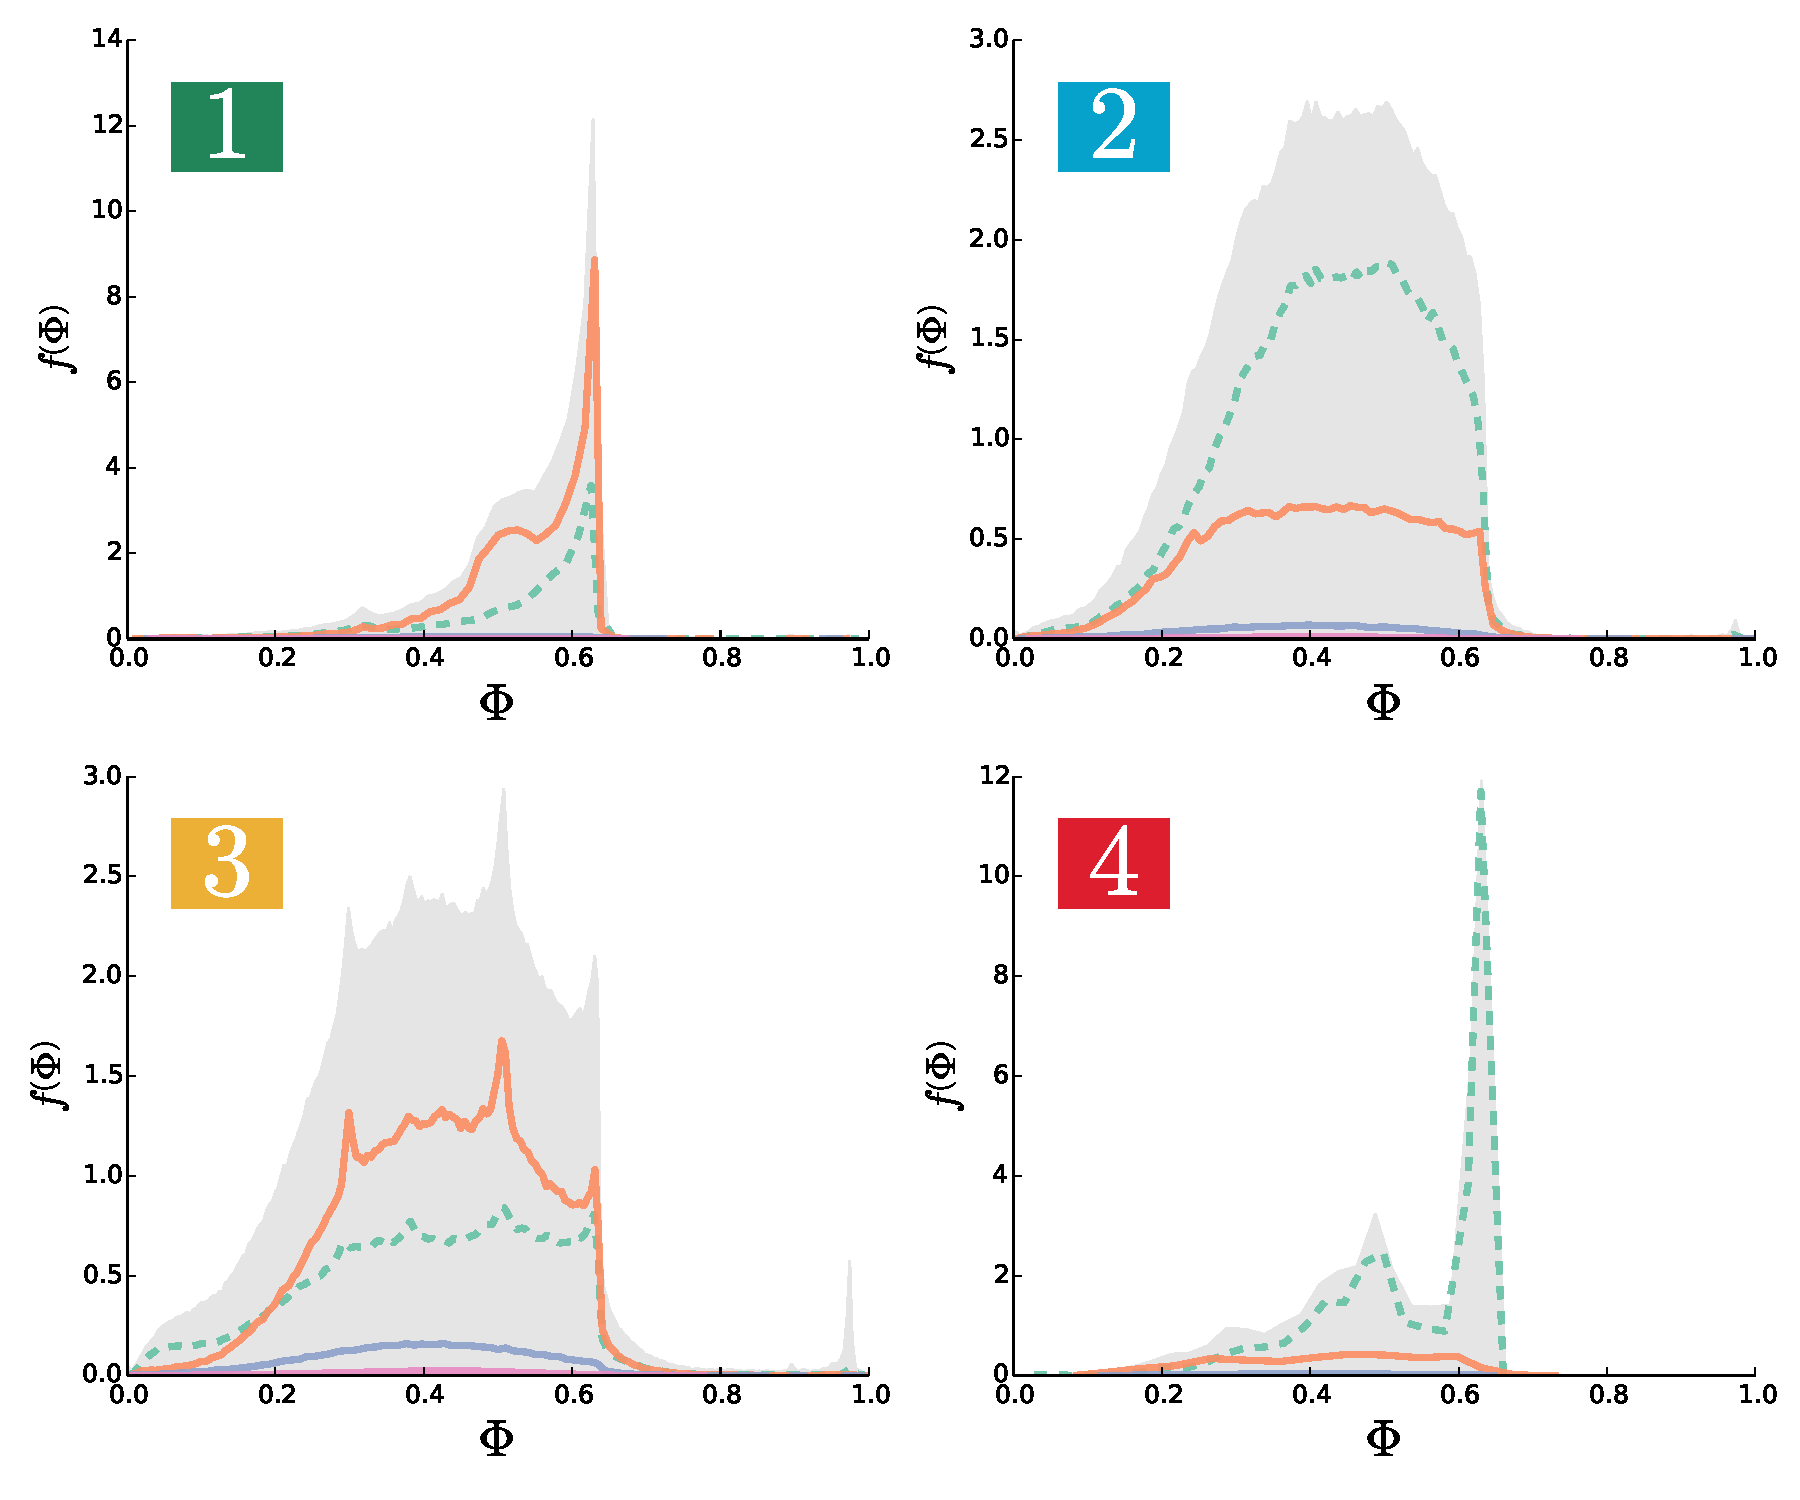
\includegraphics[height=2.1in]{./gfx/chapter-networks/groups.pdf}
    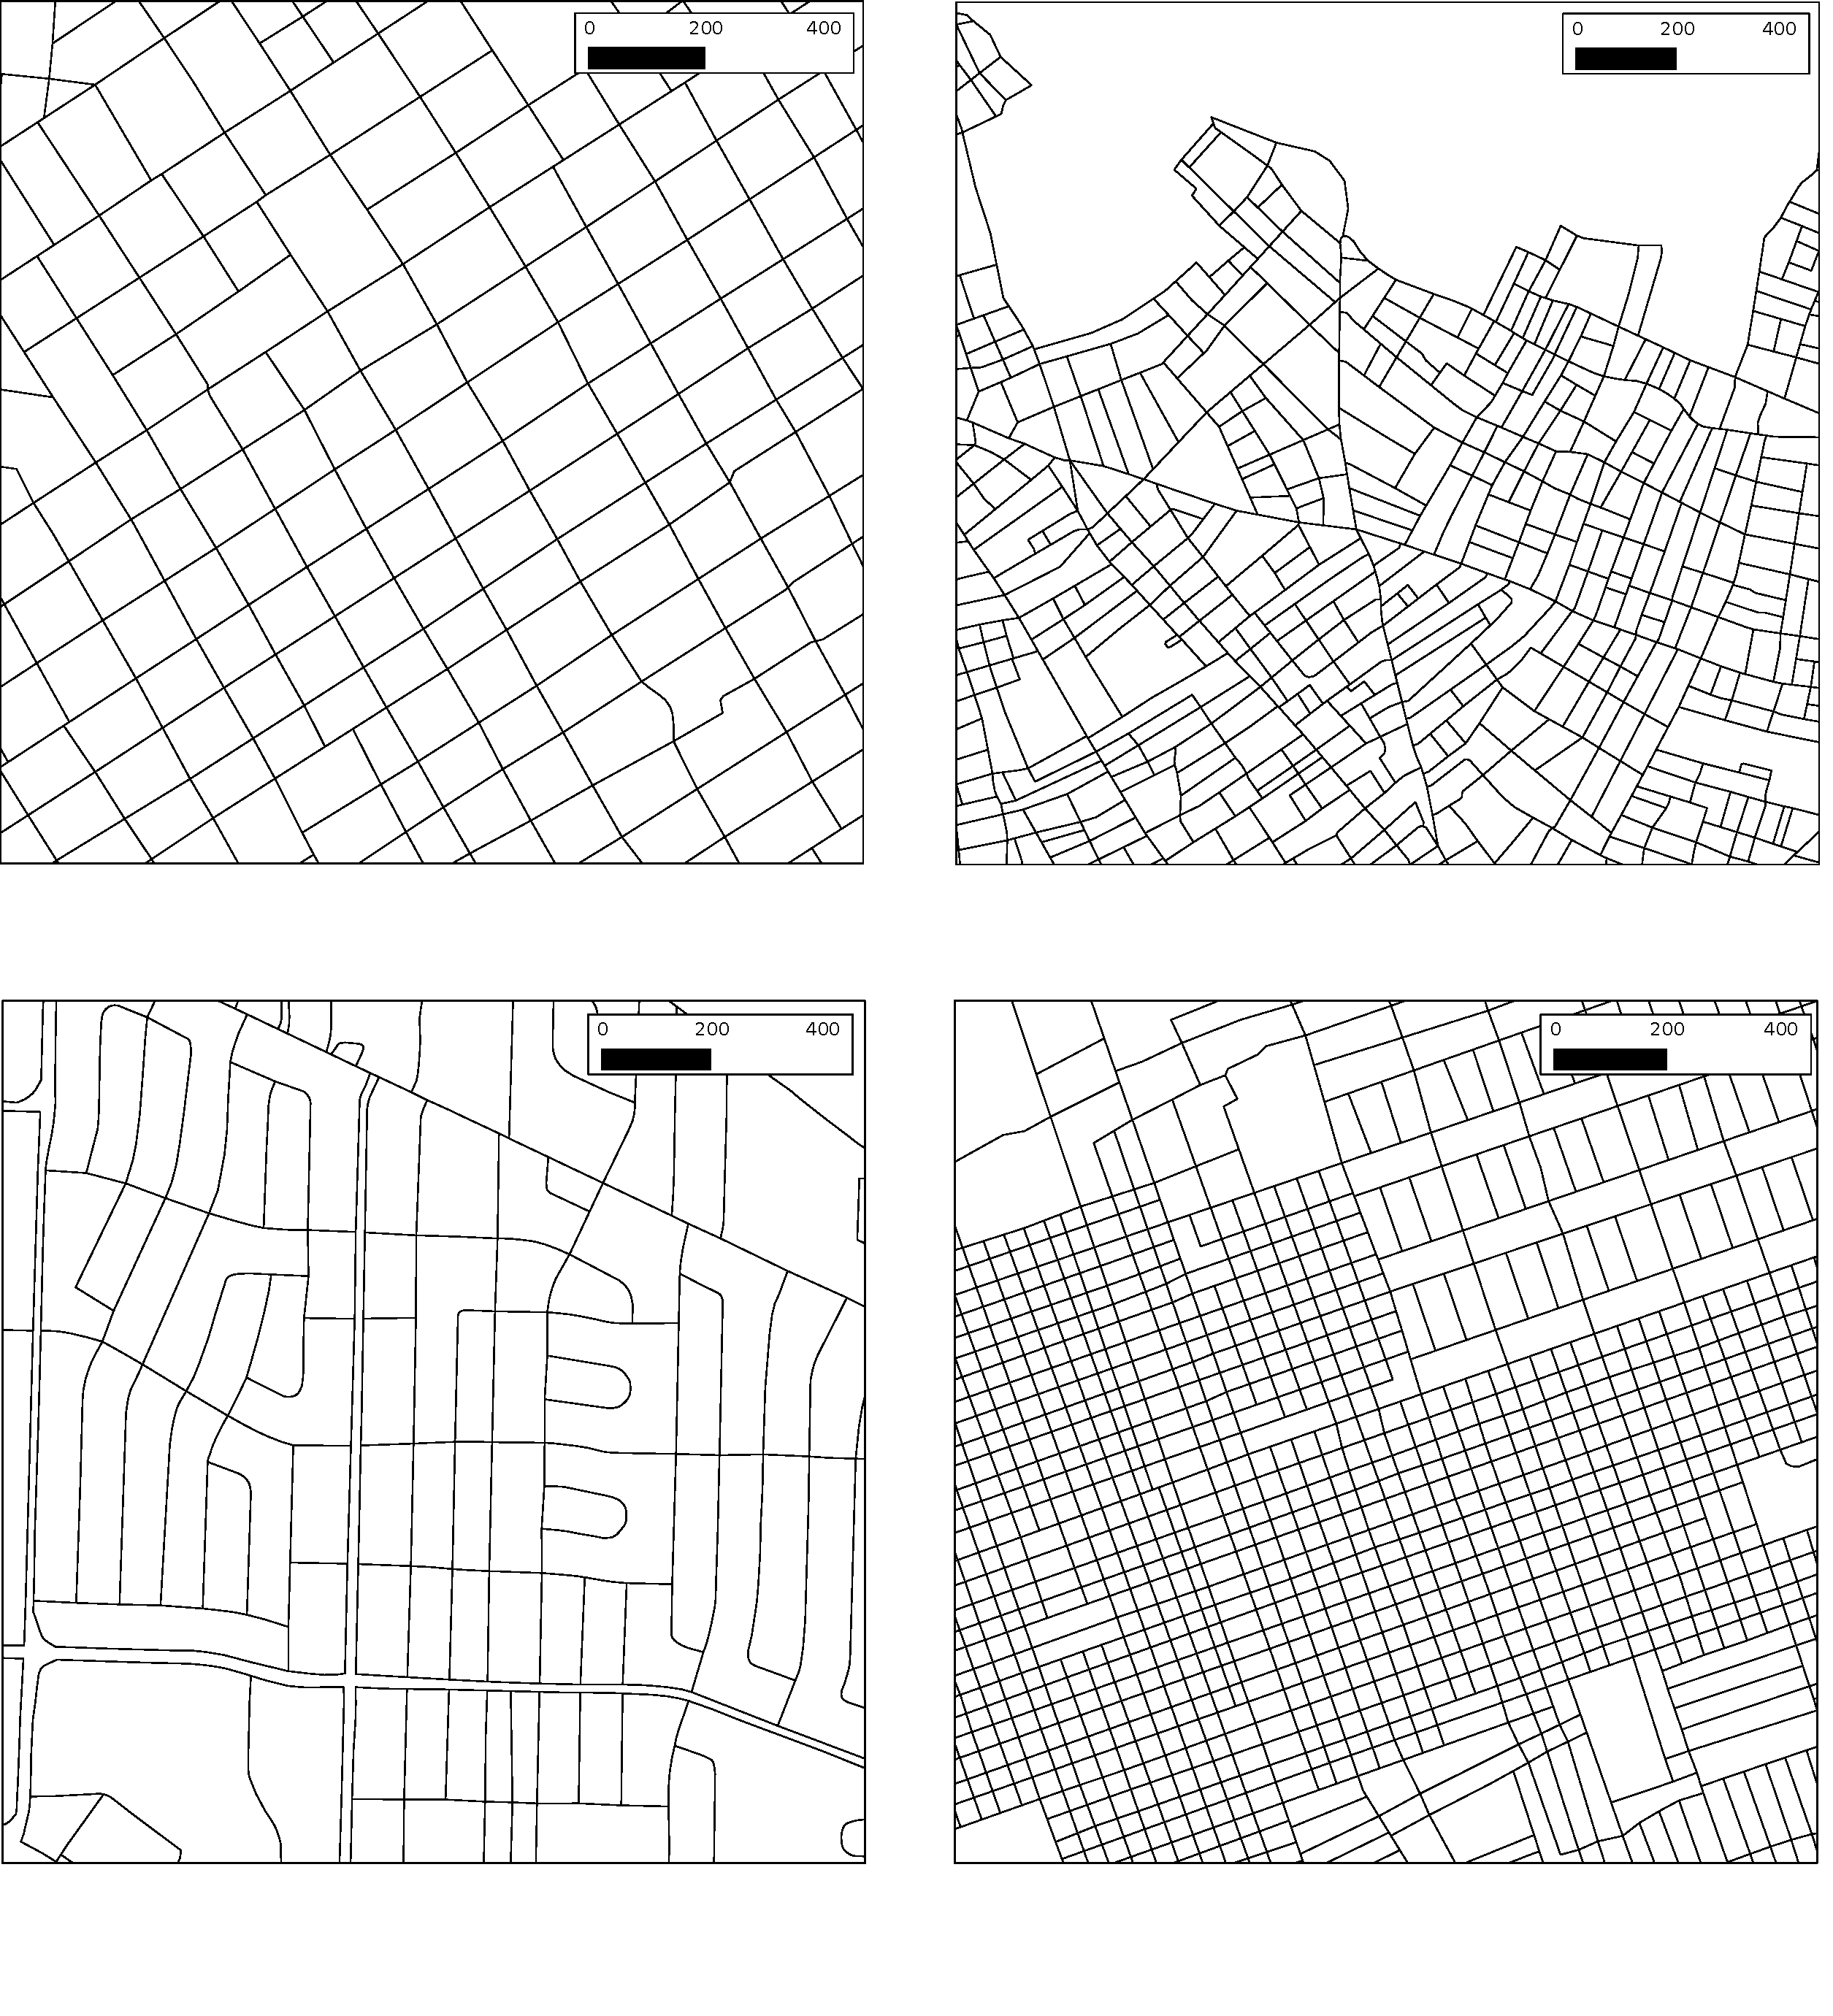
\includegraphics[height=2.1in]{./gfx/chapter-networks/groups_patterns.pdf}
    \caption{{\bf The four groups.} (Left) Average distribution of the shape
    factor $\Phi$ for each group found by the clustering algorithm (Right) Typical
    street pattern for each group (plotted at the same scale in order to observe
    differences both in shape and areas). Group 1 (top left): Buenos Aires | Group
    2: Athens | Group 3: New Orleans | Group 4: Mogadishu \label{fig:groups}}
\end{figure}

Blocks are polygons and as such can be characterized by simple measures. First,
the surface area $A$ of a block gives a useful indication, and its distribution
is an important information about the block pattern. As
in~\cite{Lammer:2006,Fialkowski:2008}, we find that for different cities the
distributions have different shapes for small areas, but display fat tails
decreasing as a power law \begin{equation} P(A)\sim \frac{1}{A^\tau}
\end{equation} with an exponent of order $\tau\approx 2$
\cite{Lammer:2006,Barthelemy:2011,Strano:2012,Barthelemy:2013,frag:2014}.
Although this seemingly universal behaviour gives a useful constraint on any
model that attempts at modeling the evolution of cities' road
networks~\cite{frag:2014}, it does not allow to distinguish cities from each
other.

A second characterization of a block is through its shape, with the form (or
shape) factor $\Phi$, defined in the Geography literature in~\cite{Hagget:1965}
as the ratio between the area of the block and the area of the circumscribed
circle $\mathcal{C}$
%
\begin{equation} \Phi = \frac{A}{A_{\mathcal{C}}} \end{equation}
%
The quantity $\Phi$ is always smaller than one, and the smaller its value, the
more anisotropic the block is. There is not a unique correspondence between a
particular shape and a value of $\Phi$, but this measure gives a good indication
about the block's shape in real-world data, where most blocks are relatively
simple polygons. The distributions of $\Phi$ displays important differences from
one city to another, and a first naive idea would be to classify cities
according to the distribution of block shapes given by $P(\Phi)$. The shape
itself is however not enough to account for visual similarities and
dissimilarities between street patterns. Indeed, we find for example that for
cities such as New-York and Tokyo, even if we observe similar distributions
$P(\Phi)$ (see Fig.~\ref{fig:fingerprint}), the visual similarity between both
cities's layout is not obvious at all. One reason for this is that blocks can
have a similar shape but very different areas: if two cities have blocks of the
same shape in the same proportion but with totally different areas, they will
look different.  We thus need to combine the information about both the shape
and the area.

\begin{figure}
    \center
    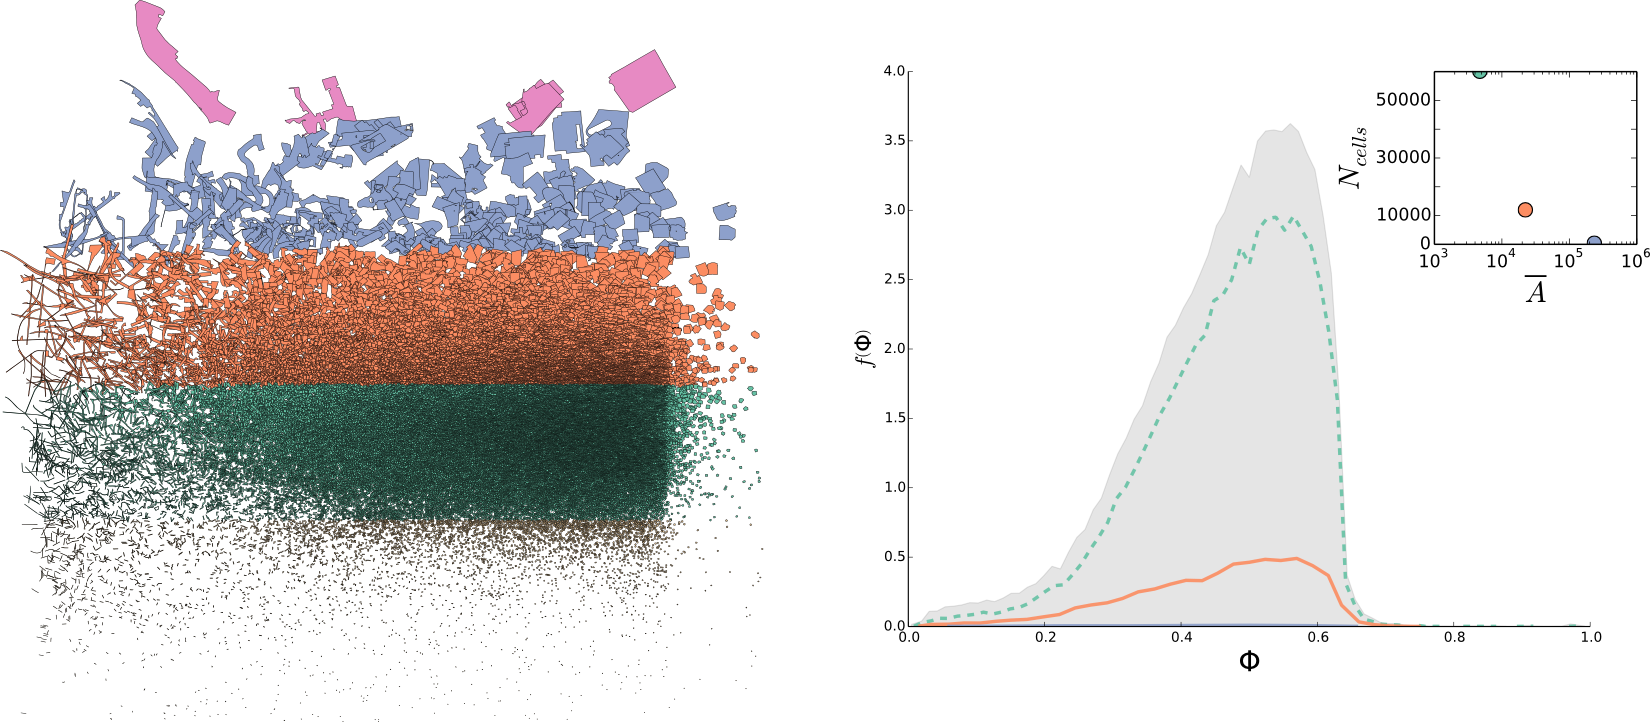
\includegraphics[width=\textwidth]{./gfx/chapter-networks/steps_tokyo.png}
    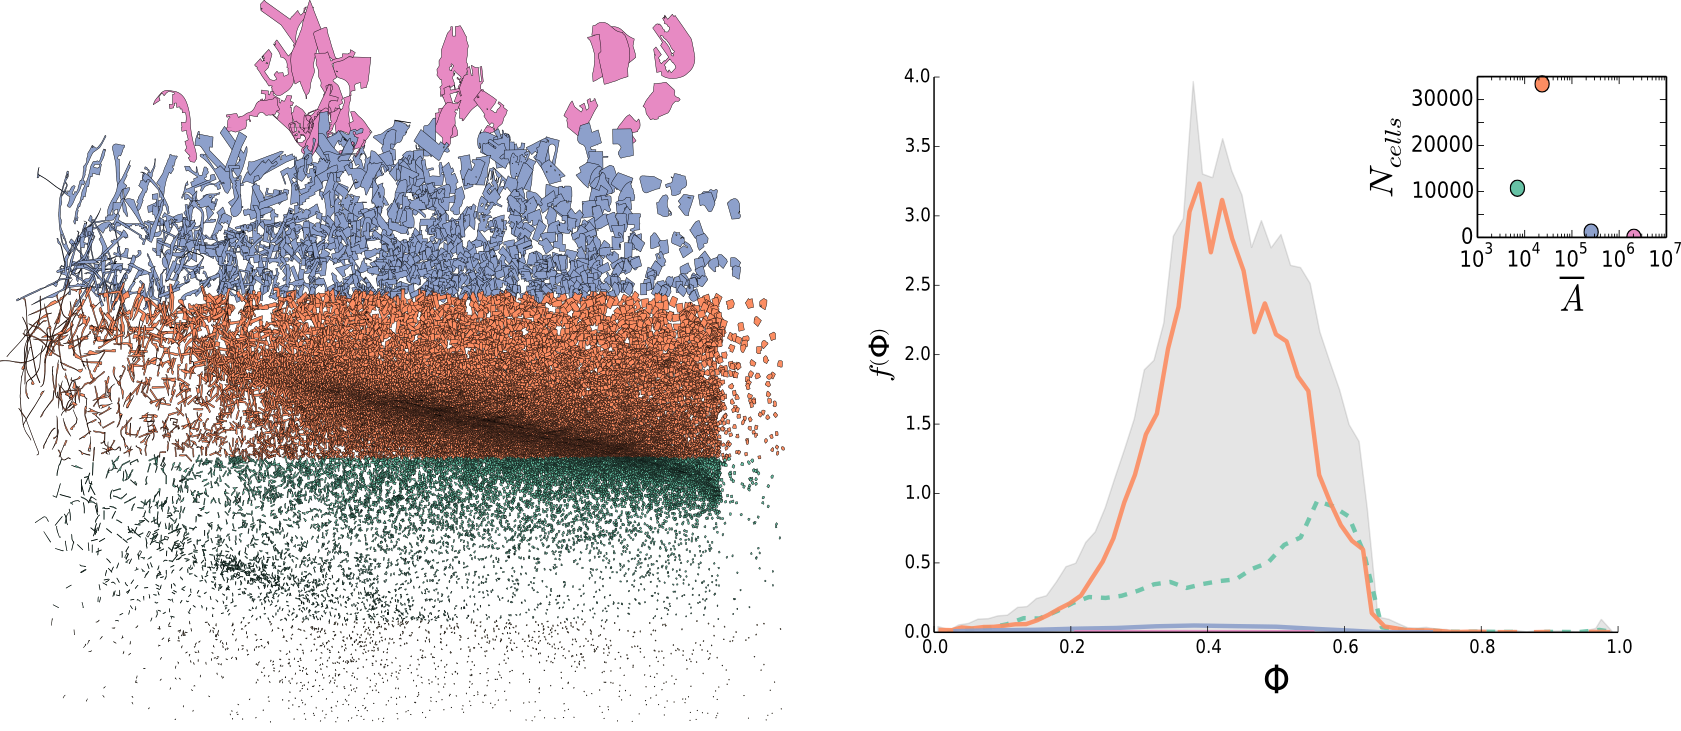
\includegraphics[width=\textwidth]{./gfx/chapter-networks/steps_ny.png}
    \caption{{\bf The fingerprints of Tokyo (top) and New-York, NY (bottom).}
    (Left) We rearrange the blocks of a city according to their area (y-axis), and
    their  $\Phi$ value (x-axis). The color of each block corresponds to the area
    category it falls into.  (Right) We quantify this pattern by plotting the
    distribution of shapes, as measured by $\Phi$ for each area category,
    represented by coloured curves. The gray curve is the sum of all the coloured
    curve and represents the distribution of $\Phi$ for all cells. As shown in the
    inset, we see that intermediate area categories dominate the total number of
    cells, and are thus enough for the clustering procedure.\label{fig:fingerprint}}
\end{figure}

In order to construct a simple representation of cities which integrates both
area and shape, we rearrange the blocks according to their area (on the y-axis)
and display their $\Phi$ value on the x-axis (Fig.~ \ref{fig:fingerprint}). We
divide the range of areas in (logarithmic) bins and the color of a block
represents the area category to which it belongs. We describe quantitatively
this pattern by plotting the conditional probability distribution $P(\Phi|A)$ of
shapes, given an area bin (Fig.~ \ref{fig:fingerprint}, right). The colored
curves represent the distribution of $\Phi$ in each area category, and the curve
delimited by the gray area is the sum of all the these curve and is the
distribution of $\Phi$ for all cells, which is simply the translation of the
well-known formula for probability conditional distribution

\begin{equation} 
    P(\Phi)=\sum_AP(\Phi|A)P(A) 
\end{equation}

These figures give a `fingerprint' of the city which encodes information about
both the shape and the area of the blocks. In order to quantify the distribution
of blocks inside a city, and thus the visual aspect of the latter, we will then
use $P(\Phi|A)$ for different area bins. The comparison between these quantities
will provide the basis for a classification of street patterns that we propose
here.


\section{A typology of cities across the world}

Two cities will display similar patterns if their blocks have both similar area
and shape. In other words, the shape distributions for each area bin should be
very close, and this simple idea allows us to propose a distance between street
patterns of different cities. More precisely, as one can see on
Fig.~\ref{fig:fingerprint}, the number of blocks of area in the range
$[10^3,10^5]$ (in square meters) dominate the total number of cells, and we will
neglect very small blocks (of area $<10^3\text{m}^2$) and very large ones (of
area $>10^5\text{m}^2$). We thus sort the blocks according to their area in two
distinct bins

\begin{align*} 
    \alpha_1 &= \left\{ \text{cells} | \mathcal{A} \in \left[10^3,
10^4\right]\right\}\\ 
    \alpha_2 &= \left\{ \text{cells} | \mathcal{A} \in
\left[10^4, 10^5\right]\right\}\\ 
\end{align*}

We denote by $f_\alpha(\Phi)$ the ratio of the number of cells with a form
factor $\Phi$ that lie in the bin $\alpha$ over the total number of cells for
that city. We then define a distance $d_\alpha$ between two cities $a$ and $b$
characterized by their respective $f^{a}_\alpha$ and $f^{b}_\alpha$

\begin{equation} 
    d_\alpha(a,b) = \int_0^1\: | f^{a}_\alpha(\Phi) -
f^{b}_\alpha(\Phi) |\: \mathrm{d}\Phi 
\end{equation} 

and we construct a global distance $D$ between two cities by combining all area
bins $\alpha$

\begin{equation} 
    D(a,b)= \sum_\alpha d_\alpha(a,b)^{\,2} 
\end{equation} 

At this
point, we have a distance between two cities' pattern and we measure the
distance matrix between all the $131$ cities in our dataset, and perform a
classical hierarchical clustering on this matrix \cite{Clustering}. We
obtain the dendrogram represented on Fig.~\ref{fig:dendrogram} and at an
intermediate level, we can identify $4$ distinct categories of cities, which
are easily interpretable in terms of the abundance of blocks with a given
shape and with small or large area. On Fig.~\ref{fig:groups} we show the
average distribution of $\Phi$ for each category and show typical street
patterns associated with each of these groups. The main features of each
group are the following.  

\begin{figure}
    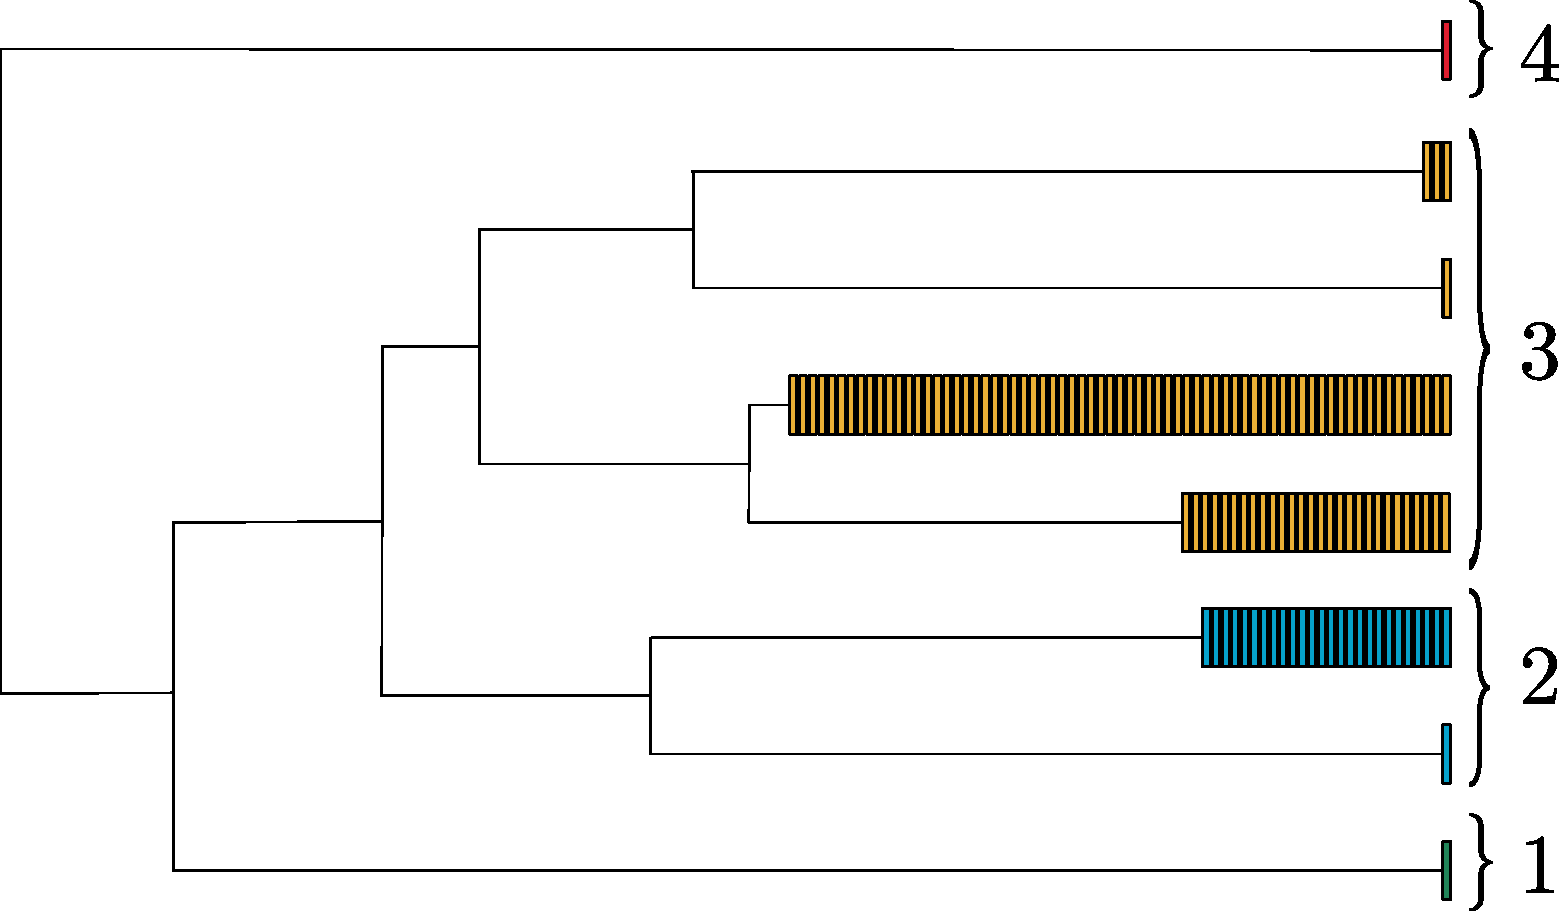
\includegraphics[width=0.75\textwidth]{./gfx/chapter-networks/dendrogram.pdf}
    \caption{{\bf Dendrogram} We represent the structure of the hierarchical
    clustering at a given level. Interestingly, $68\%$ of american cities are
    present in the second largest sub-group of group $3$ (fourth from the top).
    Also, all european cities but Athens are in the largest subgroup of the group
    $3$ (third from top). This result gives a first quantitative grounding to the
    feeling that European and most American cities are laid out
    differently.\label{fig:dendrogram}} 
\end{figure}

\begin{itemize} 
    \item{} In the group 1 (comprising
        Buenos Aires only) we essentially have blocks of medium size (in
        the bin $\alpha_2$) with shapes that are dominated by the square
        shape and regular rectangles. Small areas (in bin $\alpha_1$)
        are almost exclusively squares.  \item{} Athens is a
        representative element of group 2, which comprises cities with a
        dominant fraction of small blocks with shapes broadly distributed.
    \item{} The group 3 (illustrated here by New Orleans) is similar to the
        group 2 in terms of the diversity of shapes but is more balanced in
        terms of areas, with a slight predominance of medium size blocks.
    \item{} The group 4 which contains for this dataset the interesting
        example of Mogadishu (Somalia) displays essentially small,
        square-shaped blocks, together with a small fraction of small
        rectangles.  
\end{itemize}

The proportion and location of cities belonging to each group is shown on
Fig.~\ref{fig:world_map}. Although one should be wary of sampling bias here, it
seems that the type of pattern characteristic of the group $3$ (various shapes
with larger areas) largely dominates among cities in the world. Interestingly,
all North American cities (except Vancouver, Canada) are part of the group $3$,
as well as all European cities (except Athens, Greece). The composition of the
other continents is more balanced between the different groups. Strikingly, we
find that at a smaller scale within the group $3$ (Fig.~\ref{fig:dendrogram}),
all European cities (but Athens) in our sample belong to the same subgroup of
the group $3$ (the largest one, third from the top on
Fig.~\ref{fig:dendrogram}). Similarly, $15$ American cities out of the $22$ in
our dataset belong to the same subgroup of the group $3$ (the second largest
one, fourth from the top on Fig.~\ref{fig:dendrogram}. Exceptions are
Indianapolis (IN), Portland (OR), Pittsburgh (PA), Cincinnati (OH), Baltimore
(MD), Washington (DC), and Boston (MA), which are classified with European
cities, confirming the impression that these US cities have an european imprint.
These results point towards important differences between US and European
cities, and could constitute the starting point for the quantitative
characterization of these differences \cite{Bretagnolle:2010}.


\section{A local analysis}

Cities are complex objects, and it is unlikely that an object as simple as the
fingerprint can describe all its intricacies. Indeed, cities are usually made of
different neighbourhood which often exhibit different street patterns. In
Europe, the division is usually clear between the historical center and the more
recent surburbs. A striking example of such differences is the Eixample
neighbourhood in Barcelona, very distinct from other areas of the city. In order
to illustrate this difference, and to show that they also can be captured with
our method, we isolate the different Boroughs of New-York, NY: the Bronx,
Brooklyn, Manhattan, Queens and Staten Island. We extract the fingerprint of
each Borough, as represented on Fig.~\ref{fig:ny-boroughs}. The fingerprint of
New-York (bottom Fig.~\ref{fig:fingerprint}) is indeed the combination of
different fingerprints for each of the boroughs. While Staten Island and the
Bronx have very similar fingerprints, the others are different. Manhattan
exhibits two sharp peaks at $\Phi \approx 0.3$ and $\Phi \approx 0.5$ which are
the signature of a grid-like pattern with the predominance of two types of
rectangles. Brooklyn and the Queens exhibit a sharp peak at different values of
$\Phi$, also the signature of grid-like patterns with different rectangles for
basic shapes. 

\begin{figure}
    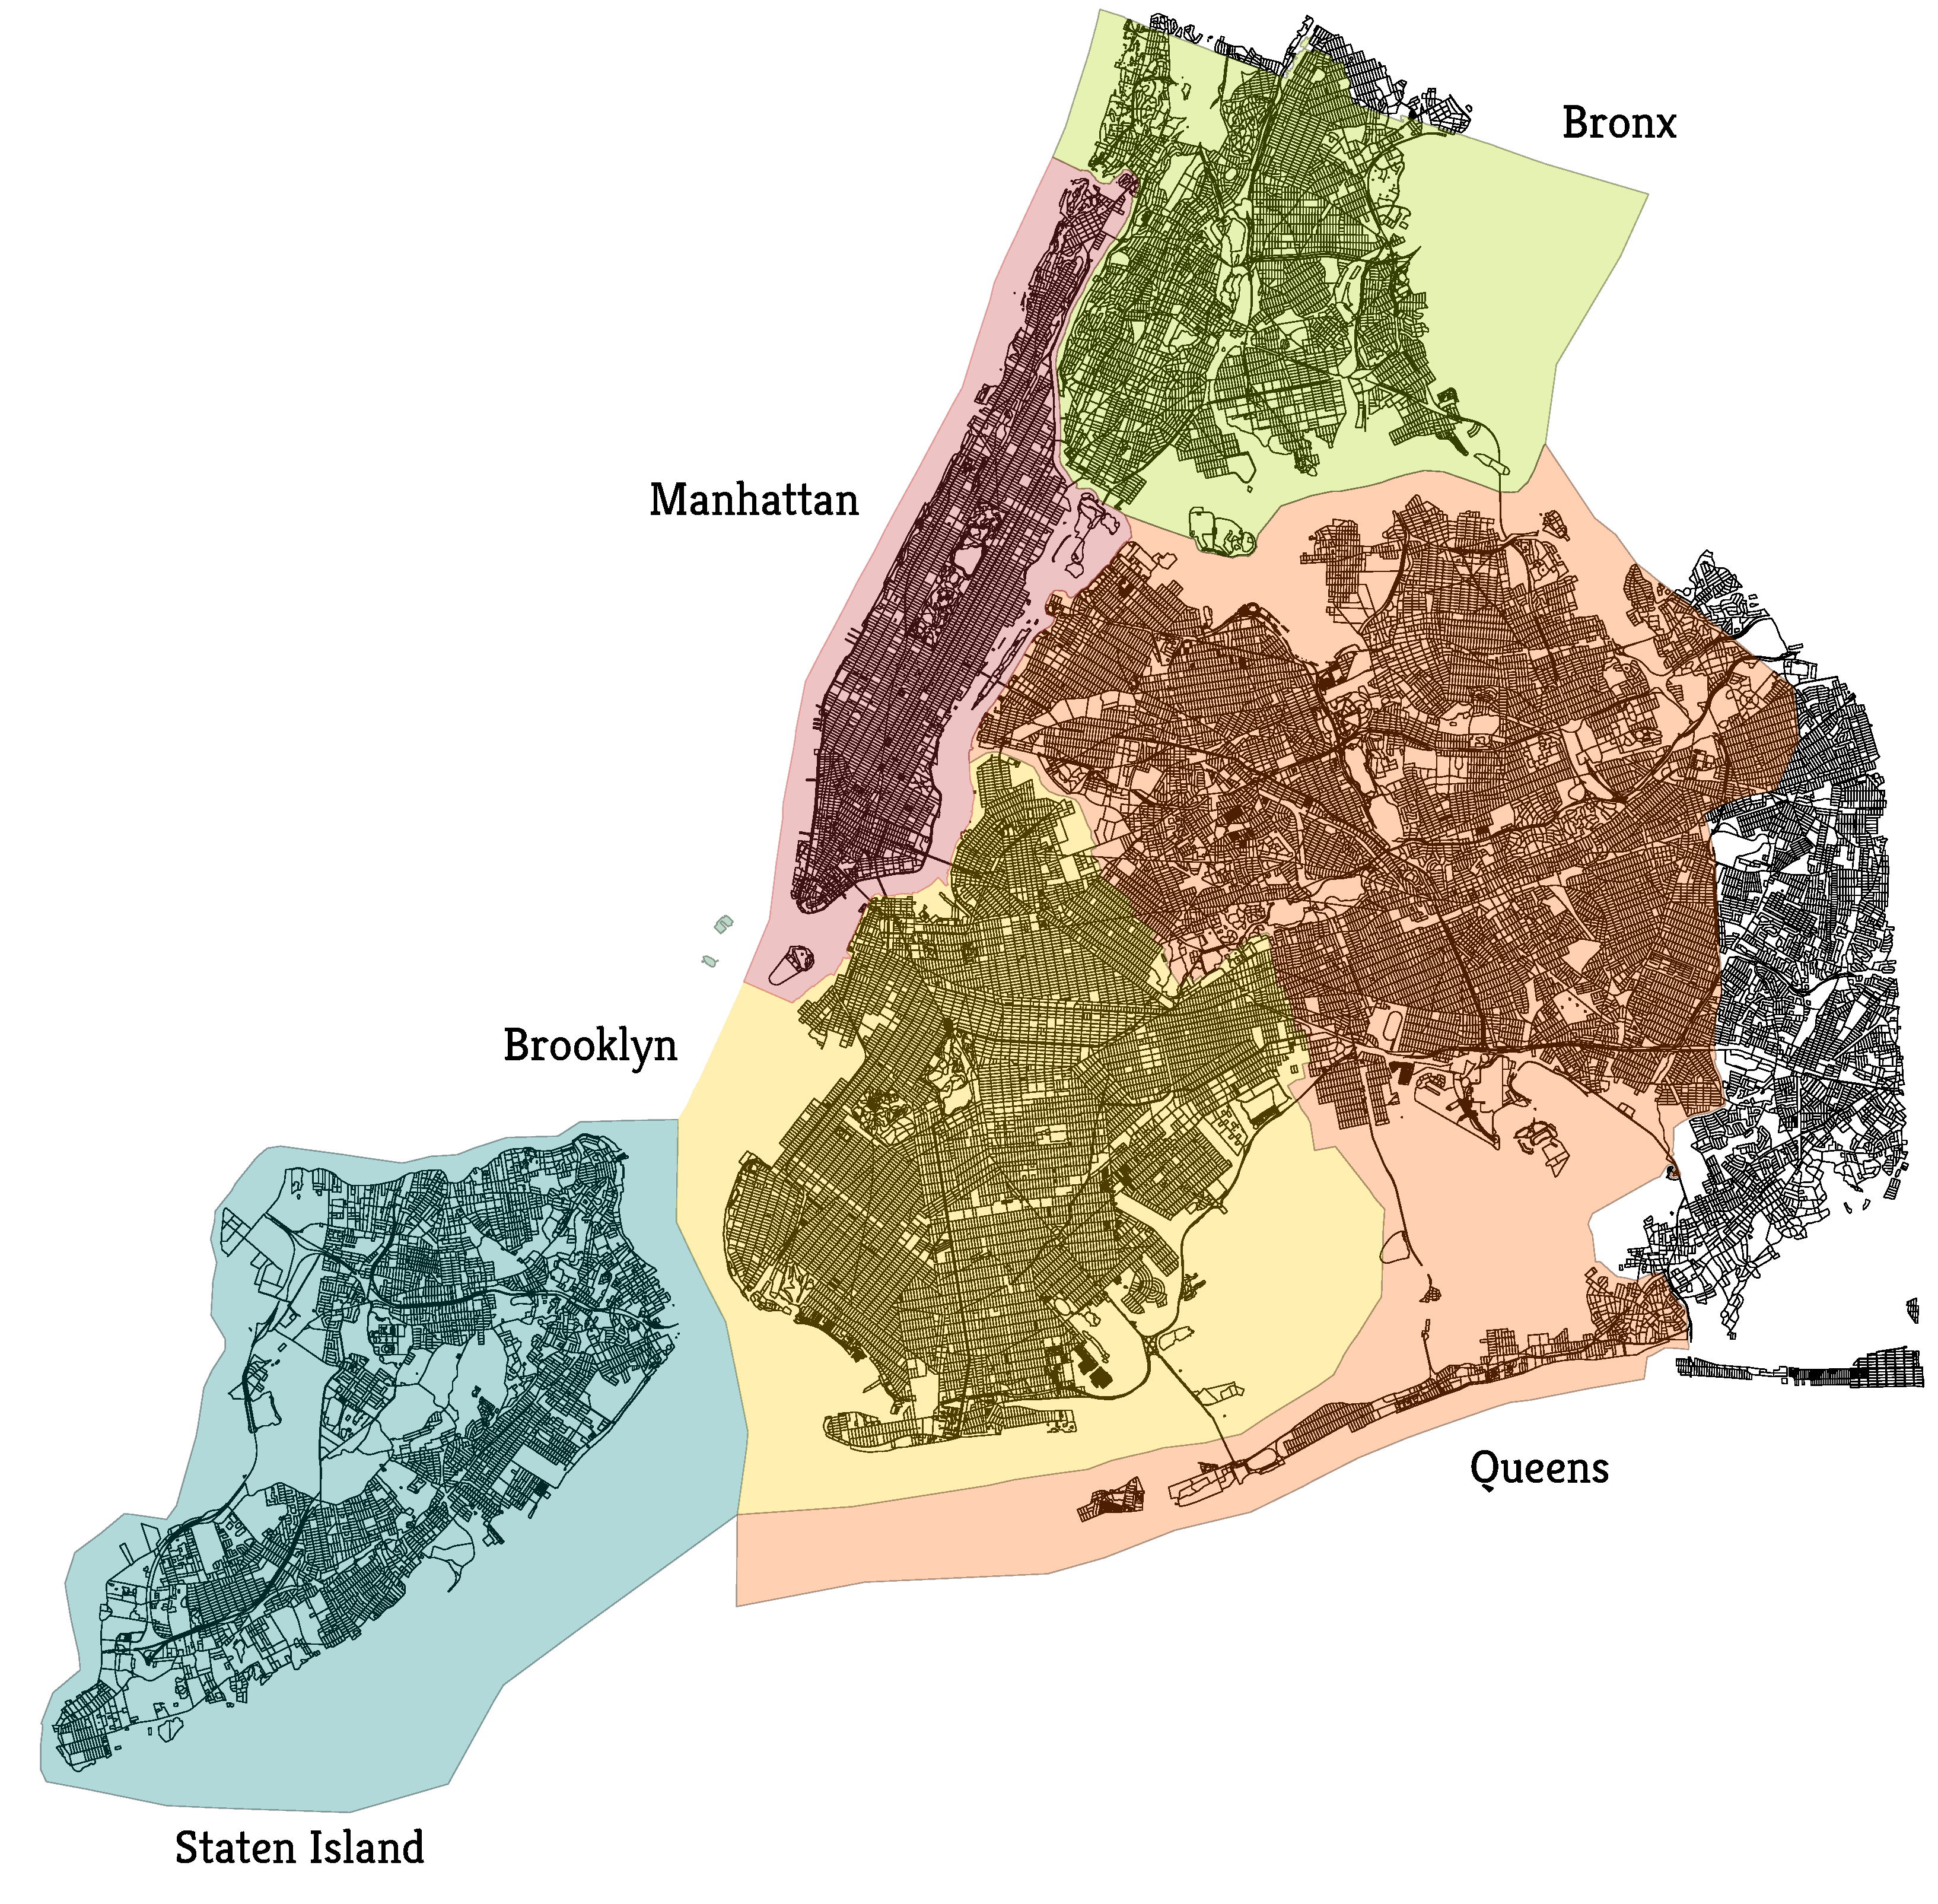
\includegraphics[height=4in]{./gfx/chapter-networks/ny_boroughs.pdf}
    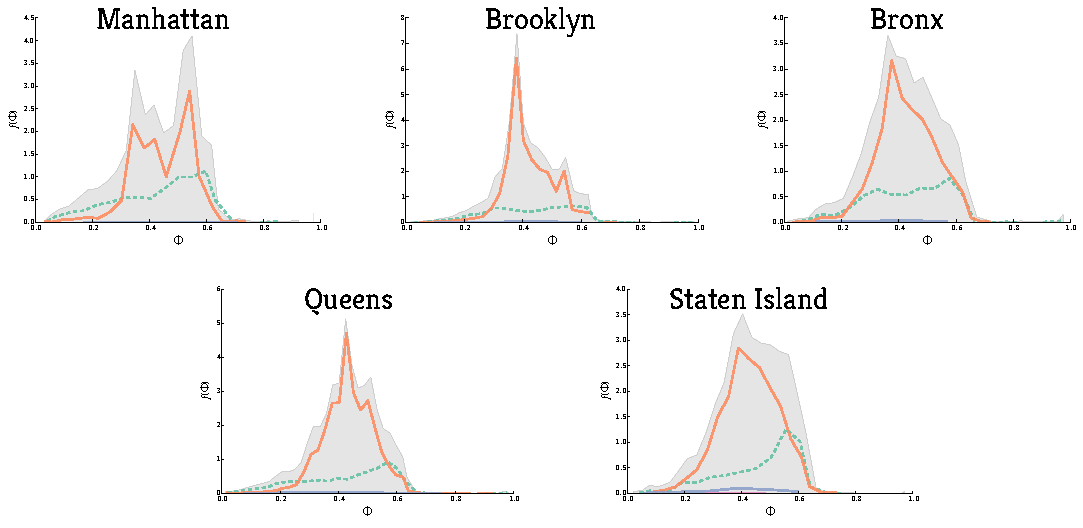
\includegraphics[width=\textwidth]{./gfx/chapter-networks/boroughs_distributions.pdf}
    \caption{{\bf New-York, NY and its different boroughs} \label{fig:ny-boroughs}
    (Top) We represent New York City and its 5 boroughs: the Bronx, Brooklyn,
    Manhattan, Queens, and Staten Island. (Bottom) The corresponding fingerprints
    for each borough. Only Staten Island and the Bronx have similar fingerprints and
    the others are different. In particular,  Manhattan exhibits two sharp peaks at
    $\Phi \approx 0.3$ and $\Phi \approx 0.5$ which are the signature of a grid-like
    pattern with the predominance of two types of rectangles. Brooklyn and the
    Queens exhibit a sharp peak at different values of $\Phi$, signalling the
    presence of grid-like patterns made of different basic
    rectangles.\label{fig:boroughs}}
\end{figure}


\section{Discussion and perspectives}

We have introduced a new way of representing cities' road network that can be
seen as the equivalent of fingerprints for cities. It seems reasonable to think
that the possibility of a classification based on these fingerprints hints at
common causes behind the shape of the networks of cities in the same categories.
Of course, the present study has limitations: even if the shape of the blocks
alone is good enough for the purpose of giving a rough classification of cities,
we miss some aspects of the patterns. Indeed, the way the blocks are arranged
together locally should also give some information about the visual aspect of
the global pattern. Indeed, many cities are made of neighbourhoods, built at
different times, with different street patterns. What is lacking at this point
is a systematic, quantitative way to identify and distinguish different
neighbourhoods, and to describe their correlation. Indeed, the Boroughs taken as
examples in the last section are administrative, arbitrary definitions of a
neighbourhood. Reality is however more complex: similar patterns might span
several administrative regions, or a given administrative division might host
very distinct neighbourhoods. A further step in the classification would thus be
to find a method to extract these neighbourhoods, and integrate the spatial
correlations between different types of neighbourhoods.

Despite the simplifications that our method entail, we believe that the
classification we propose is an encouraging step towards a quantitative and
systematic comparison of the street patterns of different cities. This, together
with the specific knowledge of architects, urbanists, etc. should lead to a
better understanding of the shape of our cities. Further studies are indeed
needed in order to relate the various types that we observe to different urban
processes. For example, in some cases, small blocks are obtained through a
fragmentation process, and their abundance could be related to the age of the
city. A large regularity of cell shapes could be related to planning such as in
the case of Manhattan for example, but we also know with the example of Paris
\cite{Barthelemy:2013} that a large variety of shapes is also directly related
to the effect of a urban modification which doesn't respect the existing
geometry.\\

Finally, we believe that important empirical progress could be made.A first
limitation of the current study is the amount of data that we have.  Although
$131$ cities is a larger number than what is used in most studies, the
OpenStreetMap database contains the street layout of many more cities. The more
cities we have, the better the classification. We should thus attempt to include
more cities.

The second limitation is the use of the administrative definition of cities to
delineate the boundaries of the street network. Administrative definitions,
because they are based on political criteria, are completely arbitrary and do
not reflect any property of the contained networks. As a result, the chosen
boundaries are likely to vary from one country to another, from one city to
another. The measures we perform on each of the $131$ are thus, strictly
speaking, not comparable. A possible solution would be to use the delineation
method proposed by Masucci et al.~\cite{Masucci:2015}, which is parameter-free
and based only on the properties of the street network.
